\documentclass[journal]{IEEEtran}
%
% If IEEEtran.cls has not been installed into the LaTeX system files,
% manually specify the path to it like:
% \documentclass[journal]{../sty/IEEEtran}

\usepackage{cite}
\usepackage[pdftex]{graphicx}
\usepackage{amsmath}
\usepackage{algorithmic}
\usepackage{array}
\usepackage[caption=false,font=footnotesize]{subfig}
\usepackage{url}
\usepackage{listings}
\usepackage{float}
\usepackage{amsfonts}
\usepackage{hyperref}
\usepackage{amssymb}
%\usepackage{fixltx2e}
%\usepackage{stfloats}


\begin{document}
\title{Estimation of Distribution using Energy-based Models}
%
%
% author names and IEEE memberships
% note positions of commas and nonbreaking spaces ( ~ ) LaTeX will not break
% a structure at a ~ so this keeps an author's name from being broken across
% two lines.
% use \thanks{} to gain access to the first footnote area
% a separate \thanks must be used for each paragraph as LaTeX2e's \thanks
% was not built to handle multiple paragraphs
%

\author{Manuela~Corte~Pause~(240183),~\IEEEmembership{University of Trento}
  and~Francesco~Gentile~(240186) ,~\IEEEmembership{University of Trento}% <-this % stops a space
}

\maketitle

\IEEEpeerreviewmaketitle

\section{Introduction}
In this work we propose a new approach for a Estimation of Distribution Algorithm (EDA) inspired by energy-based models as a way to approximate the probability distribution of a set of solutions. The proposed method, Estimation of Distribution using ENergy-based models (EDEN), is based on a neural network that approximates the energy of the population and samples from it using a modified version of Langevin dynamics.

\section{Background}
\label{sec:background}

Evolutionary Algorithms (EAs) are widely used for solving black-box optimization problems, drawing inspiration from Darwinian evolution. These algorithms operate by evolving a population of solutions through the mechanisms of selection, recombination, and mutation like for example in Genetic Algorithms (GAs) \cite{holland_ga_1992} or Evolution Strategies (ES) \cite{back_es_1996}. However, like their biological inspiration, mutation and recombination in EAs are random processes and only selection is deterministic. This randomness implies that the algorithm does not explicitly take into account the correlation between different parts of the genotype and its impact on the fitness landscape and the process is only guided by selection pressure. Consequently, the search process may be inefficient or flat out wrong in navigating deceptive fitness landscapes. If this correlation were explicitly modeled, it could potentially lead to more effective search processes.

In contrast to traditional EAs, Estimation of Distribution Algorithms (EDAs) \cite{larranaga_estimation_2002} represent a class of algorithms that aim to improve search efficiency by modeling the distribution of the best solutions discovered so far. EDAs construct a probabilistic model of the population, which is then used to generate new candidate solutions (Figure \ref{fig:eda}). By sampling from this model and selecting the best candidates, the search is guided towards more promising areas of the search space. The complexity of the dependencies modelled by the probabilistic model used can vary depending on the complexity of the optimization problem and the available computational resources. Most simple EDAs assume that the $n$-dimensional joint probability factorizes into the product of $n$ univariate distributions like in Univariate Marginal Distribution Algorithm (UMDA) \cite{muhlenbein_umda_1997}. A common approach to model more complex dependencies is to use Probabilistic Graphical Models (PGMs) like Bayesian Networks. For example Estimation of Bayesian Networks Algorithm (EBNA) \cite{larranaga_ebna_2000} constructs a Bayesian Network to model the population starting from an edge-less graph and adding edges based on some statistical test while Bayesian Optimization Algorithm (BOA) \cite{pelikan_boa_2005} uses the Bayesian-Dirichlet metric to compare the score of Bayesian Networks that encode the same conditional independency relationships.

\begin{figure}
    \centering
    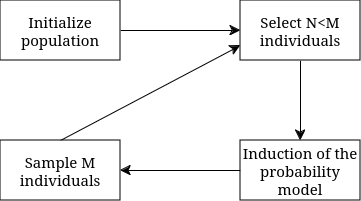
\includegraphics[width=0.3\textwidth]{img/eda.png}
    \caption{Estimation of Distribution Algorithm (EDA)}
    \label{fig:eda}
\end{figure}

Another possible approach is to use Markov Networks to model the dependencies between variables \cite{shakya_markov_2012}. A Markov Networks is a type of probabilistic graphical model represented as a pair $(G, \Psi)$, where $G$ is an undirected graph and $\Psi$ is the parameter set of the model. Unlike the more common Bayesian Networks, Markov Networks are undirected PGM and thus do make any assumption about the direction of the dependencies between variables (and thus do not have a notion of causality). While this allows to factorize a broader class of probability distributions\footnote{Note, however, that there are probability distributions that can be modelled by Bayesian Networks but not Markov Networks.}, it also makes the structure and parameter learning as well as inference more complex.

A Markov Network is characterized by two key properties:
\begin{enumerate}
    \item \textit{Local Markov property (Markovianity)}: A variable is conditionally independent of all other variables, given its neighbors (also known as the Markov blanket).
          \begin{equation*}
              P(x_i | x - \{x_i\}) = P(x_i | x_{\text{ne}(i)})
          \end{equation*}

    \item \textit{Global Markov property}: the joint probability distribution can be factorized as the product of the potential functions defined over the cliques of the graph.
          \begin{align*}
              P(x) & = \frac{1}{Z} \prod_{i=1}^m \psi_i(c_i) = \frac{1}{\sum_{x \in \Omega} \prod_{i=1}^m \psi_i(c_i)} \prod_{i=1}^m \psi_i(c_i) \\
          \end{align*}
          where $Z$, the partition function, is a normalization constant and usually intractable to compute. Equivalently, the joint distribution can be expressed using a Gibbs/Boltzmann distribution:
          \begin{equation*}
              P(x) = \frac{1}{Z} e^{-U(x)/T} = \frac{1}{\sum_{y \in \Omega} e^{-U(y)/T}} e^{-U(x)/T}
          \end{equation*}
          Here, $T$ is the temperature, and $U(x)=\sum_{i=1}^m u_i(c_i)$ represents the energy of the distribution.
\end{enumerate}

Both the local and global property can be exploited to model the population in an EDA. For example, in Markovianity based Optimization Algorithm (MOA) \cite{shakya_moa_2011} Shakya et al. first estimate the structure of the network by computing mutual information between every pair of variables. Then, by exploiting the local Markov property, they can directly sample from the underlying distribution without the need to perform parameter estimation.

On the other hand, Distribution Estimation using Markov Random Fields (DEUM) \cite{shakya_deum_2012} first estimates the network structure using statistical tests to determine the independency relationships between variables, then they try to learn the parameters so as to increase the probability of the best solutions in the population. Since naive parameter estimation would require to compute the partition function, they assume that each solution in the search space has a probability proportional to its fitness:

\begin{equation*}
    p(x) = \frac{f(x)}{Z} = \frac{f(x)}{\sum_{y \in \Omega} f(y)}
\end{equation*}

Then, by exploiting the global Markov property and equating the empirical density of a solution to the one of the model, they show that fitting the parameters of the model can be transformed into a simple regression problem:

\begin{align*}
    p(x) = \frac{f(x)}{\sum_{y \in \Omega} f(y)} & = \frac{e^{-U(x)/T}}{\sum_{y \in \Omega} e^{-U(y)/T}} \\
    -\log f(x)                                   & = U(x)
\end{align*}

Besides expressing the joint probability distribution of Markov Networks, the Boltzmann distribution is also the foundation of energy-based models \cite{teh_ebm_2003}, which are a class of models that define a probability distribution over the data by assigning an energy $E(x)$ to each configuration $x$.
\begin{equation*}
    p(x) = \frac{1}{Z_{\theta}} e^{-\beta E_{\theta}(x)}
\end{equation*}
This approach offers great flexibility, as any function (e.g., a neural network) can be used to model the energy of the distribution. However, a significant challenge arises from the normalization constant $Z_{\theta} = \int_{x \in X} -e^{-\beta E_{\theta}(x)} dx$, which is usually intractable. The standard method for learning a probabilistic model $p_{\theta}(x)$ is to maximize the expected log-likelihood of the data \cite{song_ebm_2021}:
\begin{equation}
    \mathcal{L}(\theta) = \mathbb{E}_{x \sim p_{\text{data}}(x)}[\log p_{\theta}(x)]
\end{equation}
Because of the intractability of the normalization constant, the expected log-likelihood is usually approximated using Markov Chain Monte Carlo (MCMC) approaches. One of the most widely used MCMC methods is Langevin dynamics \cite{parisi_langevin_1980}, which leverages the fact that the gradient of the log-probability is equal to the negative gradient of the energy:
\begin{align*}
    x_{t+1} & = x_t + \frac{\epsilon}{2} \nabla E(x_t) + \sqrt{2 \epsilon} z_i                  \\
            & = x_t - \frac{\epsilon}{2} \nabla \log p(x) + \sqrt{2 \epsilon} \mathcal{N}(0, I)
\end{align*}

\section{Proposed Method}
\label{sec:proposed_method}

The method hereby presented is based on the idea of approximating the probability distribution of a set of solutions using an energy-based model. In particular, we exploit the remarkable approximation capabilities of neural networks to estimate the fitness of a solution set. By also treating the neural network as an energy-based model, we can then equate the fitness of a solution to the energy computed by the model\footnote{In this work, we want to minimise the fitness function rather than maximise it as it was done in the original DEUM paper.}. Then, to minimise the Kullback-Leibler divergence between the empirical distribution of the population and the model, we can simply train the model by minimizing the Mean Squared Error (MSE) between the predicted energy and the actual fitness of the population. Furthermore, we can easily sample from the model using Langevin dynamics.

Hereafter, we will describe the two main components of the proposed method: the energy-based model and the local sampling. The energy-based model can be further divided into three sub-components: gene embeddings, structure learning and energy regressor.

\begin{figure}[H]
    \centering
    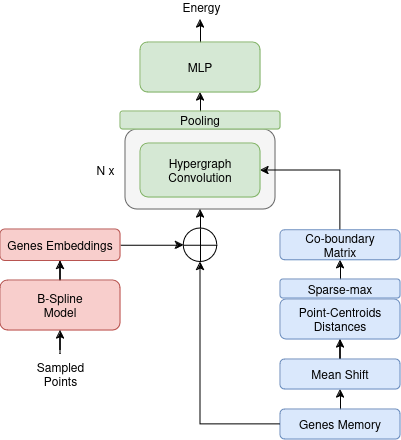
\includegraphics[width=0.35\textwidth]{img/model.png}
    \caption{Proposed architecture}
    \label{fig:method}
\end{figure}

\subsection*{Gene Embeddings}

As stated above, the energy-based model is used to predict the fitness of a solution $\mathbf{x} \in \mathbb{R}^n$ represented as a vector of $n$ genes. While it would be possible to directly use the genes values as input to the model, it has been shown in many domains that neural networks can benefit from transforming floating point values into vectorial representations.

As Langevin dynamics requires to compute the gradient of the energy with respect to the input, traditional encodings, like sinusoidal or gamma encodings, would not be suitable as they multiply the input by an exponential function, making the gradient too large. For this reason, we propose to use learnable B-spline functions to map each gene value to a higher-dimensional space. In particular this mapping is done as a weighted summation:
\begin{equation*}
    \mathbf{g}(\mathbf{x}_j) = \sum_{i=0}^n \mathbf{p}_i N_{i,m}(\mathbf{x}_j)
\end{equation*}
where $\mathbf{x}_j$ is the j-th gene, $\mathbf{p}_j$ are the learnable n-dimensional control points and $N_{i,m}$ are B-spline functions.

A B-spline of order $m+1$ is a series of piece-wise polynomial functions $N_{i,m}(t)$ of degree $m$. The points $T=t_0, t_1, \dots, t_m$, where these polynomials intersect, are known as knots and are typically placed equidistantly. A B-spline is recursively defined as follows:
\begin{align*}
    N_{i,0}(t) & = \begin{cases}
                       1 & \text{if } t_i \leq t < t_{i+1} \\
                       0 & \text{otherwise}
                   \end{cases}                                                                   \\
    N_{i,m}(t) & = \frac{t - t_i}{t_{i+m} - t_i} N_{i,m-1}(t) + \frac{t_{i+m+1} - t}{t_{i+m+1} - t_{i+1}} N_{i+1,m-1}(t)
\end{align*}
\subsection*{Structure Learning}

Following the idea of multivariate EDAs, we aim to learn the dependencies between genes to better model the fitness landscape for those problems where the genes exhibit epistasis. To do so, we view each gene as a node in a graph and we learn to cluster genes that exhibit high dependencies, thus effectively moving from a graph to a hypergraph representation.

To learn the hypergraph structure, we associate to each gene a learnable memory vector $\mathbf{m}_i \in \mathbb{R}^d$ that should encode the gene's role in the problem structure. The idea is that during the training process, genes that are dependent on each other will be pushed closer in the embedding space and thus will be clustered together.

To do so, we use mean-shift on the genes memories to compute the cluster centroids $\mathbf{C} \in \mathbb{R}^{k \times d}$, where $k$ is the number of clusters found. We then compute the cosine distance between the genes' memories and the returned centroids, obtaining a soft membership matrix that we row-wise normalize to 1. While multiple normalization functions could be used (simple summation, softmax, etc.), we choose to use the entmax-2 function \cite{martins_sparsemax_2016} as it guarantees sparsity in the output.

The resulting normalized matrix can then be considered the co-boundary matrix of the hypergraph $\mathbf{B} \in \mathbb{R}^{n \times k}$, indicating for each gene the hyperedges it belongs to.

\subsection*{Energy Regressor}

The energy regressor uses the gene embeddings and the hypergraph structure to estimates the fitness of the input individual.

Here we take a different approach from traditional undirected graphical models. In these models, the energy of a configuration is computed as the sum of the potential functions, where each potential function is defined only over the nodes of the corresponding clique. Thus, there is no direct interaction between the nodes of different cliques or between cliques themselves. Opposite to this approach, we believe that the fitness of a solution is also influenced by the interactions between groups of genes, and not only by the interactions within each group. For this reason, we propose to stack multiple hypergraph convolutional layers \cite{bai_hypergraph_2019} to allow each node to exchange information with all the other nodes in the hypergraph while still preserving the hypergraph structure.

In particular, the embeddings given in input to the first layer are computed as the sum of the gene embeddings and the gene memories that serve as a sort of positional embeddings, i.e. $\mathbf{Z}^0 = \mathbf{E} + \mathbf{M}$. Then, the embeddings are passed through multiple hypergraph convolutional layers, where the output of the $l$-th layer is computed as:

\begin{equation*}
    \mathbf{Z}^{l} = \sigma(\mathbf{B}\mathbf{B}^\intercal \mathbf{Z}^{l-1} \mathbf{W}^{l})
\end{equation*}

where $\sigma$ is the activation function and $\mathbf{W}^{l}$ is the weight matrix of the $l$-th layer.

The embedding of the input solution is then obtained by applying a permutation-invariant pooling function to the output of the last layer. In this work, we use mean-pooling, but other pooling functions could be used as well. To compute the final energy of the solution, the pooled embeddings are passed through a multi-layer perceptron (MLP) with a single output neuron:

\begin{equation*}
    E(x) = \text{MLP}(\text{pool}(\mathbf{Z}^{L}))
\end{equation*}

\subsection*{Local Sampling}

As the energy-based model is trained to approximate the fitness landscape, sampling from it can be used to obtain the more promising solutions as they have lower energy and thus higher probability. However, we found that simply applying Langevin dynamics to the model can lead to poor results. Indeed, if the fitness landscape is multimodal or very smooth, million of samples are needed to find the global optima.

To address this issue, we propose to use a modified version of Langevin dynamics that uses an adaptive noise parameter (instead of a static one) $\eta$:

\begin{equation*}
    x_{t+1} = x_t - \epsilon \nabla E(x_t) + \eta \cdot \mathcal{N}(0, I)
\end{equation*}

that can be used to bias the sampling process to stay within a region centered aroung the starting point $x_0$.

At each iteration of the optimization process, we sample a new batch of points using Langevin dynamics and the points generated in the previous iteration as starting points. We then cluster the generated points using mean-shift and we consider the clusters centroids as the basins of attraction around which we generate new points. In particular, the generation is performed by sampling from a multivariate normal distribution whose parameters are fitted on the cluster's points. Furthermore, to focus the exploration on the more promising areas of the search space, we generate for each cluster a number of points inversely proportional to the average energy of its original points.

Finally, we adjust the noise size of each cluster based on a base noise $\lambda$, the cluster extension $\delta$ and how much the cluster fitness has improved from the previous iteration:

\begin{align*}
    \delta(C_{i,t}) & = \max_{i} x_i - \min_{i} x_i \forall x \in C_{i,t}                                                                        \\
    \phi(C_{i,t})   & = \begin{cases}
                            \sqrt{f(C_{i,t}) / f(C_{i, t-1}) } & \text{if } \exists C_{i, t-1} \sim C_{j,t} \\
                            1                                  & \text{otherwise}                           \\
                        \end{cases} \\
    \eta_i          & = \lambda \delta(C_{i,t}) \phi(C_{i,t})
\end{align*}

To determine whether the fitness of a cluster has improved, we need to match the clusters from the current iteration to the clusters from the previous iteration. To do so, we compute the inter-cluster distance between each pair of new and old clusters. If no distance is below a certain threshold, the cluster is considered new, otherwise, it is matched to the closest cluster.

The adaptive noise parameter is a form of trade-off between exploration and exploitation: if the cluster has improved and became more compact, the noise is reduced, allowing the search to focus on the found optima. On the other hand, if the cluster has not improved or has expanded, the noise is increased, incentivizing exploration of different areas.

\begin{figure}
    \centering
    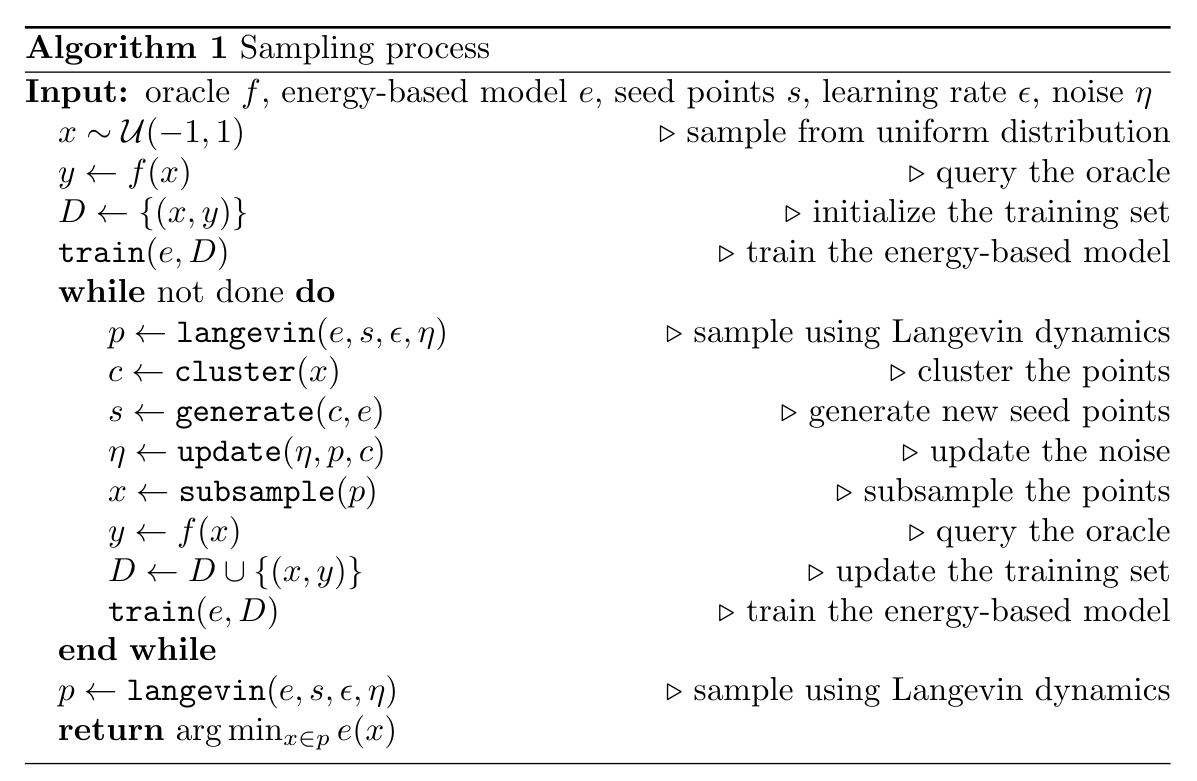
\includegraphics[width=\columnwidth]{img/sampling.png}
    \caption{Sampling process}
    \label{alg:sampling}
\end{figure}

From the algorithm above (see Figure \ref{alg:sampling}), one can see that differently from EDAs, the new parameters of the model are not fitted only on the new best sampled points, but on the whole history of the sampling process. This is necessary as neural networks suffer from catastrophic forgetting and poor out-of-distribution generalization. If we were to train the model only on the new points, it may start assigning low energy to the old points, thus making the search go back to the same regions.

\section{Results and Discussion}
\label{sec:results}

We evaluated the performance of EDEN on a series of benchmark functions to assess its effectiveness on optimization problems of varying complexity. Initially, we verified the correctness of the method using the Sphere, a simple unimodal function. Subsequently, we tested EDEN on more challenging multimodal functions, including the Rastrigin, Ackley, and Griewank functions, all within a 100-dimensional search space.


The method performances were compared against a standard Genetic Algorithm (GA) \cite{holland_ga_1992} and the Covariance Matrix Adaptation Evolution Strategy (CMA-ES) algorithm \cite{hansen_cma_2001}. All methods where compared over 10,000 fitness evaluations and the results are shown in Table \ref{tab:results} and Figures \ref{fig:sphere}, \ref{fig:rastrigin}.

\begin{table}[H]
    \centering
    \caption{Best fitness found by each algorithm on the benchmark functions}
    \begin{tabular}{|c|c|c|c|}
        \hline
        Function  & EDEN     & GA       & CMA-ES    \\
        \hline
        Sphere    & 1.049    & 85.972   & 7.931e-14 \\
        Rastrigin & 251.234  & 1010.571 & 57.073    \\
        Ackley    & 4.981e-3 & 4.953    & 3.532e-7  \\
        Griewank  & 5.974    & 435.020  & 3.731e-6  \\
        \hline
    \end{tabular}
    \label{tab:results}
\end{table}

\begin{figure}
    \centering
    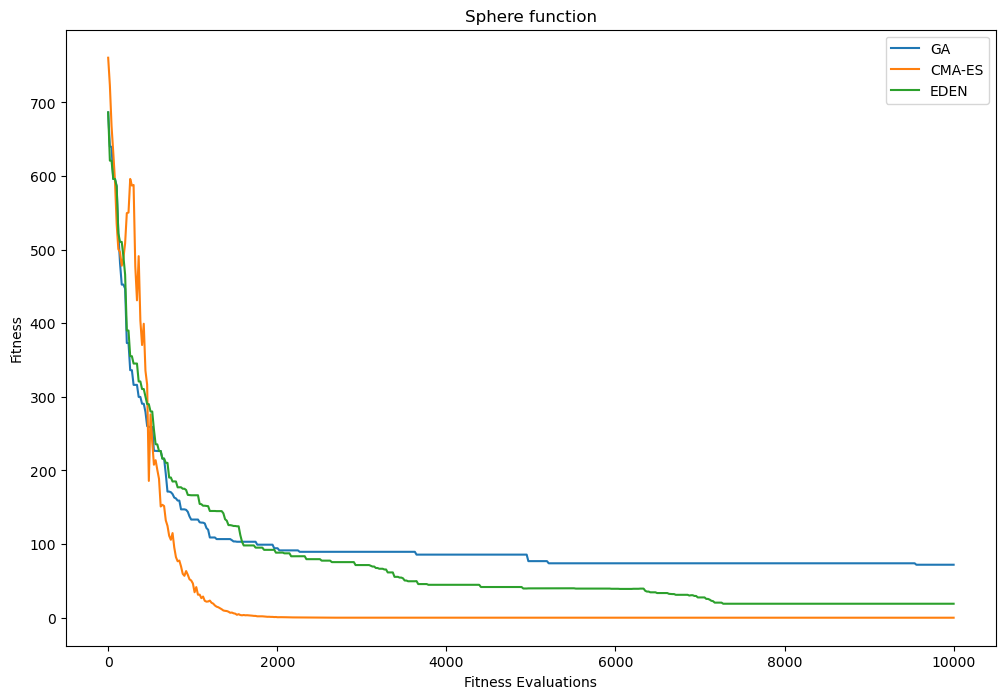
\includegraphics[width=0.4\textwidth]{img/sphere.png}
    \caption{Comparison on the Sphere function}
    \label{fig:sphere}
\end{figure}

\begin{figure}
    \centering
    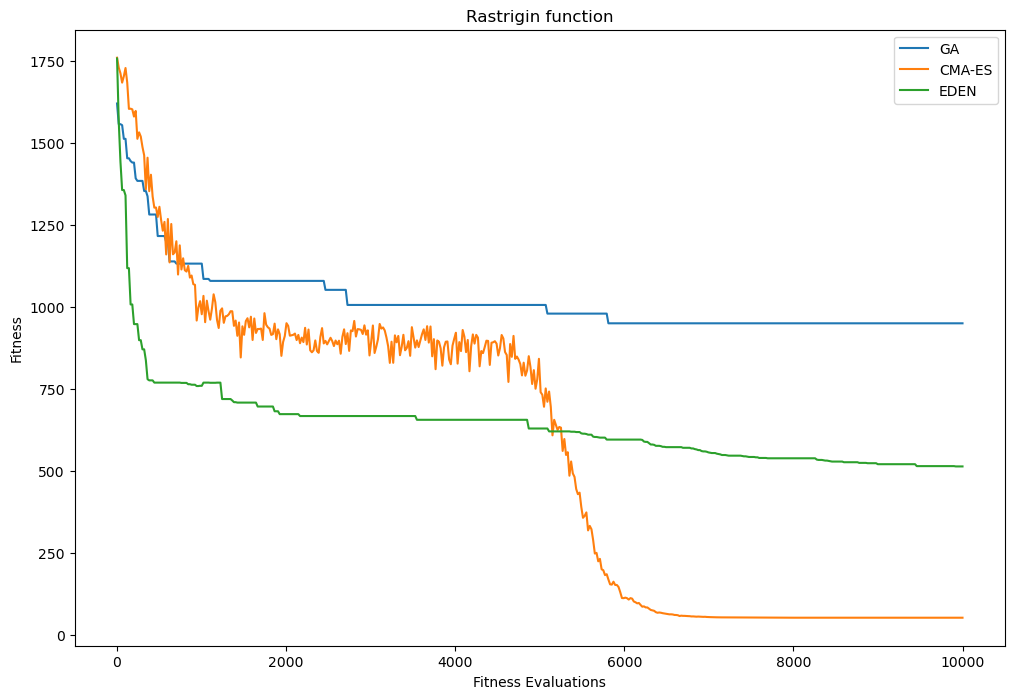
\includegraphics[width=0.4\textwidth]{img/rastrigin.png}
    \caption{Comparison on the Rastrigin function}
    \label{fig:rastrigin}
\end{figure}

The results indicate that CMA-ES consistently outperforms the other algorithms across all benchmarks. While EDEN surpasses the GA in all cases, it still lags behind CMA-ES. Interestingly, EDEN struggled more with the Sphere function than expected, despite its relative simplicity.

The poor performances of EDEN are likely not due to the fitting abilities of the model itself, but a consequence of the sampling method. Langevin dynamics performance is heavily dependent of the choice of the learning rate and the noise parameter. Even with an adaptive noise parameter to help focusing the sampling on increasingly smaller areas, we found the method still struggles to focus on a specific region thus hindering the convergence to the global optimum.

% \subsection{Possible Improvements}
% Testing the method on deceptive benchmark functions, such as the trap function, could provide deeper insights into its ability to exploit epistasis. For instance, MOA \cite{shakya_moa_2011} uses the binary trap5 function as a deceptive benchmark:
% \begin{align*}
%     f_{trap,k}(x) = \sum_{i=1}^{n/k}trap_{k}(x_{b_i,1} + \ldots + x_{b_i,k}) \\
%     trap_{k}(u) = \begin{cases}
%                       f_{high}                          & \text{if } u = k \\
%                       f_{low}   - u \frac{f_{low}}{k-1} & \text{otherwise}
%                   \end{cases}
% \end{align*}
% where $u$ is the number of ones in the input block of $k$ bits, and $f_{high}$ and $f_{low}$ are parameters that control the distance between the local and global optima.

% Additionally, expanding the analysis to include comparisons with other EDA algorithms would provide valuable insights into EDEN’s relative performance and identify potential areas for improvement.


% \appendices
% \section{Proof of the First Zonklar Equation}
% Appendix one text goes here.


\ifCLASSOPTIONcaptionsoff
  \newpage
\fi

% references section

% can use a bibliography generated by BibTeX as a .bbl file
% BibTeX documentation can be easily obtained at:
% http://mirror.ctan.org/biblio/bibtex/contrib/doc/
% The IEEEtran BibTeX style support page is at:
% http://www.michaelshell.org/tex/ieeetran/bibtex/
\bibliographystyle{IEEEtran}
\bibliography{references.bib}
% argument is your BibTeX string definitions and bibliography database(s)
%\bibliography{IEEEabrv,../bib/paper}
%
% <OR> manually copy in the resultant .bbl file
% set second argument of \begin to the number of references
% (used to reserve space for the reference number labels box)
% \begin{thebibliography}{1}

%   \bibitem{IEEEhowto:kopka}
%   H.~Kopka and P.~W. Daly, \emph{A Guide to \LaTeX}, 3rd~ed.\hskip 1em plus
%   0.5em minus 0.4em\relax Harlow, England: Addison-Wesley, 1999.

% \end{thebibliography}

\end{document}
